%!TeX program = xelatex
\documentclass{SYSUReport}
\usepackage{amsmath}
\usepackage{tikz}
\usepackage{tikz-qtree}
\usepackage{adjustbox} % 加入调整表格大小的宏包
\usepackage{booktabs} % 用于创建更漂亮的表格
\usepackage{multirow} % 用于合并单元格
\usepackage{graphicx}
\usepackage{longtable}
\usepackage{amsmath}

\usepackage{listings}
\usepackage{xcolor}

\lstdefinestyle{mystyle}{
    backgroundcolor=\color{gray!10},      % 背景色
    basicstyle=\ttfamily\small,           % 基本字体
    keywordstyle=\color{blue!70!black},   % 关键字颜色
    commentstyle=\color{green!40!black},  % 注释颜色
    stringstyle=\color{purple!60!black},  % 字符串颜色
    numbers=left,                         % 行号
    numberstyle=\tiny\color{gray},
    frame=single,                         % 边框
    breaklines=true,                      % 自动换行
    captionpos=b                          % caption 在底部
}

\lstset{style=mystyle}


% 根据个人情况修改
\headl{学号 姓名}
\headr{数据安全和隐私保护}
\lessonTitle{数据安全和隐私保护}
\reportTitle{数据安全和隐私保护实验一：实验基础工具使用}
\stuname{姓名}
\stuid{学号}
\inst{网络空间安全学院}
\major{网络空间安全}
% 修改为具体日期
\date{2026 年 9 月 10 日}

\begin{document}

\cover
\thispagestyle{empty} % 首页不显示页码
\clearpage


\tableofcontents
\clearpage


\pagenumbering{arabic}
\setcounter{page}{1}

\section{实验要求}

\subsection{实验目标}

熟练掌握相关实验工具的使用。通过本实验，使学生掌握基本的科研代码管理方法，了解 AI 辅助编程工具的使用流程，并养成规范保存代码和撰写实验报告的习惯。

\subsection{实验题目}

本实验主要围绕科研过程中常用的基础工具展开，包括：

\begin{itemize}
    \item Git 与 GitHub 代码管理，包括代码上传、下载与更新；
    \item Codex AI 编程工具的安装、配置与基本使用；
    \item LaTeX 报告的写作规范。
\end{itemize}

\subsection{实验要求}

\begin{enumerate}
    \item 了解 LaTeX 中图片插入的基本方法，并在实验报告中实际插入至少一张实验结果图。实验过程中尽量使用 PDF、SVG、EPS 等矢量图片，避免直接使用低分辨率截图作为论文或实验报告中的结果图；并要掌握 \verb|\includegraphics| 的基本使用方法，并能够合理设置图片大小；图片应包含规范的图编号、图标题，并在正文中进行引用。本部分主要作为后续实验报告撰写的基础要求，不要求进行复杂的 LaTeX 排版实践。
    \item 掌握 Git 和 GitHub 的基本使用方法，能够完成代码仓库的创建、克隆、提交、上传和更新。学生需安装并配置 Git，然后使用 GitHub 建立个人实验代码仓库，git push 本地代码到远程仓库。
    \item 完成 Codex 的安装和基本配置，下载并配置 cc-switch，对供应商进行配置与切换，并使用 Codex 完成至少一次任务（代码阅读、生成或修改）。
    \item 本次实验中，git、codex、cc-switch 之前就已经安装和配置好的同学可以跳过安装和配置过程，仅完成其他部分即可，注意实验报告中别泄露自己的 api key。
    \item 实验报告需包含必要的操作步骤、关键命令、过程截图、代码修改情况及实验总结。尽量使用 LaTeX 模版编写实验报告。
    \item 实验报告提交时间：9 月 24 日 12:00 之前（交给助教）。
\end{enumerate}

\section{实验原理}

\subsection{Git 与 GitHub}

Git 是分布式版本控制系统，本地工作区保存正在编辑的文件，暂存区保存准备提交的变化，\texttt{commit} 把暂存内容记录到本地仓库，\texttt{push} 将本地提交上传到远程仓库（如 GitHub），\texttt{pull} 将远程更新拉取并合并到本地。其基本流程为：

\begin{center}
\begin{tabular}{c}
工作区 $\xrightarrow{\text{\texttt{git add}}}$ 暂存区 $\xrightarrow{\text{\texttt{git commit}}}$ 本地仓库 $\xrightarrow{\text{\texttt{git push}}}$ GitHub \\
GitHub $\xrightarrow{\text{\texttt{git pull}}}$ 本地仓库与工作区
\end{tabular}
\end{center}

其中 \texttt{status} 用于判断当前状态，\texttt{diff} 用于比较内容差异，\texttt{log} 用于追溯提交历史，三者都是提交前后的核对工具。

\subsection{Codex AI 编程工具}

Codex 是 OpenAI 提供的 AI 辅助编程命令行工具（CLI）。它能在用户授权范围内读取项目、修改文件并运行本地工具，根据自然语言需求和仓库上下文制定并执行操作。生成结果仍可能存在错误、遗漏或不安全修改，因此可靠流程应包含权限确认、命令审阅、程序运行、测试和 Git 差异检查。

\subsection{CC Switch 供应商管理}

CC Switch 是第三方开源桌面工具，用于管理 Codex 等命令行工具的供应商配置。它把不同供应商的端点、模型和认证配置保存为可切换条目：普通切换通过更新 Codex 的配置文件生效；本地代理接管则把 Codex 请求先发送到本机代理，再由代理转发到当前供应商。v3.20.1 起第三方切换采用 config-only 模式，密钥写入 Codex 配置的 \texttt{model\_providers} 表中，不再进入 \texttt{auth.json}。

\subsection{LaTeX 图片排版}

位图由像素组成，放大后可能出现锯齿或模糊；矢量图保存曲线、文字和几何对象，缩放时通常仍能保持清晰。科研图表优先导出为 PDF/SVG 等矢量格式。LaTeX 通过 \texttt{graphicx} 宏包将图片按版面尺寸排入文档，\texttt{caption} 负责图题，\texttt{label} 与 \texttt{ref} 建立正文引用。

\section{实验设置}

\begin{table}[htbp]
\centering
\caption{实验软硬件环境}
\label{tab:env}
\begin{tabular}{lll}
\toprule
\textbf{类别} & \textbf{名称} & \textbf{版本 / 说明} \\
\midrule
操作系统 & Windows 11 & 10.0.26200 \\
代码管理 & Git & 2.45.1.windows.1 \\
脚本语言 & Python & 3.9.13（Anaconda）\\
AI 编程工具 & Codex CLI & 0.154.0（npm 全局安装）\\
供应商管理 & CC Switch & v3.20.1（Windows 便携版）\\
绘图工具 & matplotlib & 用于生成矢量实验结果图 \\
报告排版 & SYSUReport 模板 & ctexart / XeLaTeX 编译 \\
\bottomrule
\end{tabular}
\end{table}

实验仓库创建于本地，采用 \texttt{git init -b main} 初始化，远程仓库以本地裸仓库（\texttt{git init --bare}）模拟 GitHub 远程，操作流程与真实 GitHub 一致；Codex 在线任务通过 CC Switch 切换到国内可直连的 DeepSeek 供应商后完成（详见第 4.3 节），最终代码与报告均推送至真实 GitHub 仓库。

\section{实验过程}

\subsection{LaTeX 图片排版}

本部分按照规范完成 LaTeX 图片排版练习：

\begin{enumerate}
    \item 将图片统一放入 \texttt{figures} 目录，文件名使用简短英文、数字和下划线，例如 \texttt{wordfreq.pdf}；
    \item 在导言区加载 \texttt{graphicx} 宏包（模板已加载），在正文中插入图片、标题和标签；
    \item 在正文中使用“如图 \ref{fig:wordfreq} 所示”引用图片，编译后检查文字、曲线和图例是否清晰。
\end{enumerate}

本实验对词频统计程序（见 4.2 节）的运行结果进行了可视化：使用 Python matplotlib 将 \texttt{sample.txt} 中前 10 个高频词绘制为柱状图，并直接导出为 PDF 矢量图，插入结果如图 \ref{fig:wordfreq} 所示。

\begin{figure}[htbp]
    \centering
    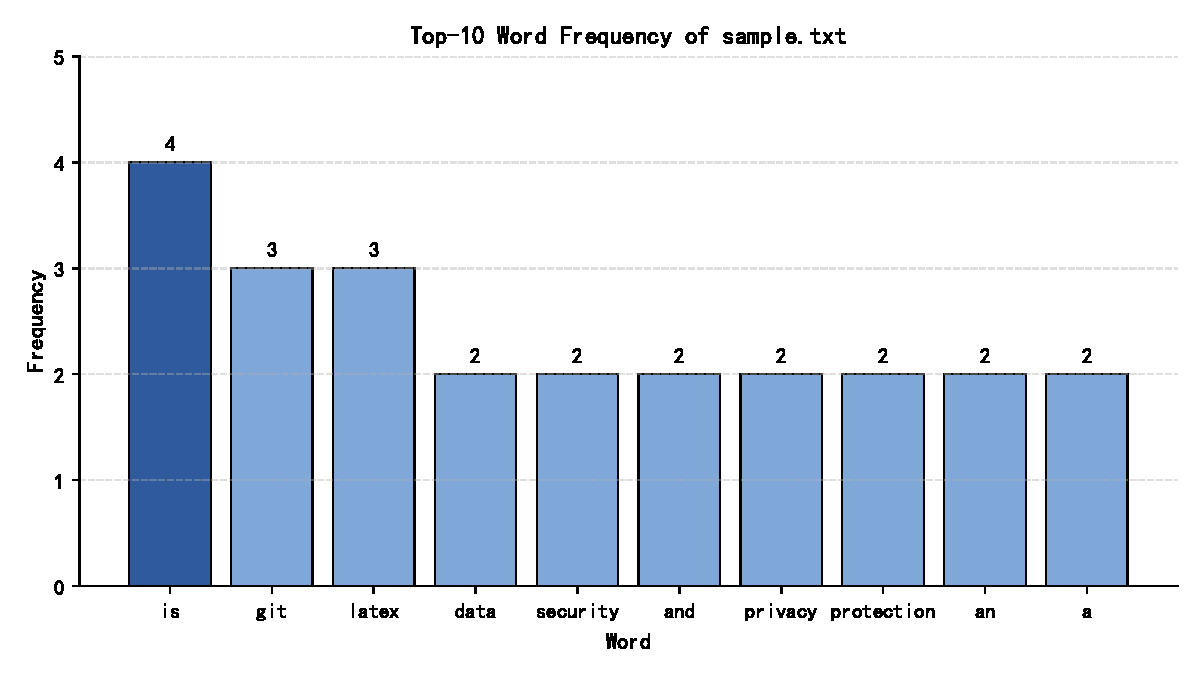
\includegraphics[width=0.85\textwidth]{figures/wordfreq.pdf}
    \caption{词频统计实验结果（Top-10 高频词，矢量 PDF 图）}
    \label{fig:wordfreq}
\end{figure}

LaTeX 插入图片的代码示例：

\begin{lstlisting}[language=TeX, caption={LaTeX 图片插入示例}]
\usepackage{graphicx}               % 导言区加载宏包
\begin{figure}[htbp]
  \centering
  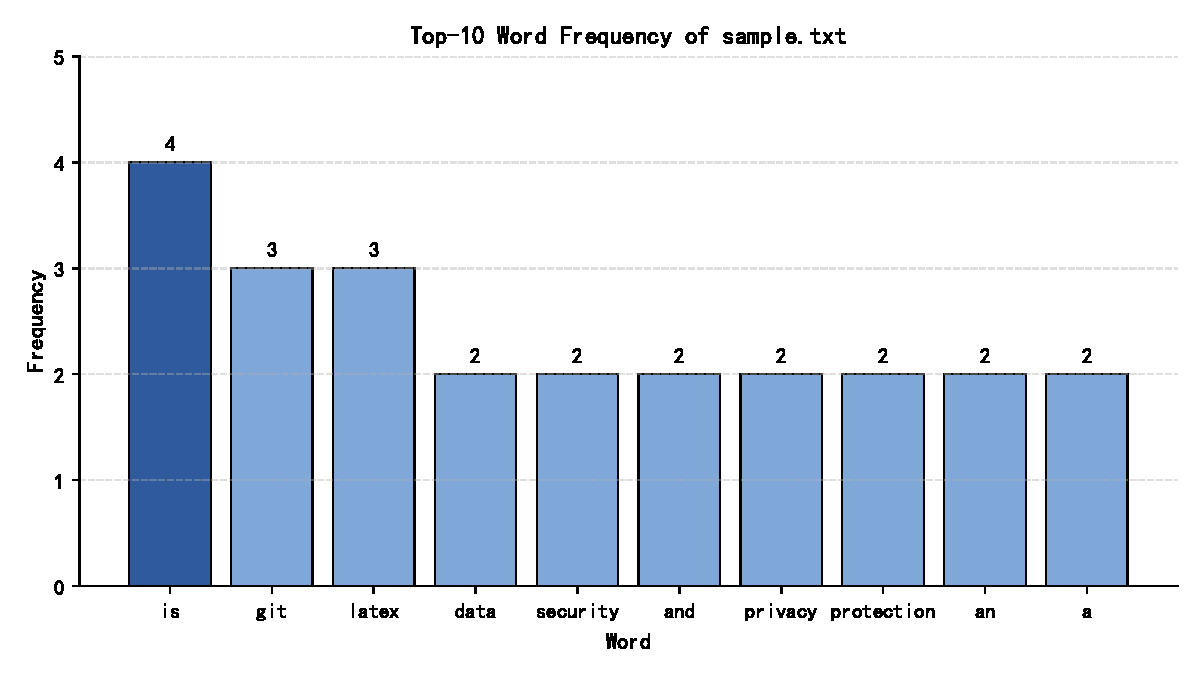
\includegraphics[width=0.85\textwidth]{figures/wordfreq.pdf}
  \caption{词频统计实验结果}
  \label{fig:wordfreq}
\end{figure}
% 正文中引用：如图 \ref{fig:wordfreq} 所示
\end{lstlisting}

\subsection{Git 和 GitHub 使用}

\subsubsection{环境确认与配置}

Git 已安装，先确认版本并核对全局身份配置：

\begin{lstlisting}[caption={Git 版本与全局配置}]
$ git --version
git version 2.45.1.windows.1

$ git config --global user.name "Freya Xu"
$ git config --global user.email "3872642750@qq.com"
$ git config --global --list --show-origin
file:C:/Users/xrl05/.gitconfig  user.name=Freya Xu
file:C:/Users/xrl05/.gitconfig  user.email=3872642750@qq.com
\end{lstlisting}

\subsubsection{创建仓库并下载代码}

在实验目录创建仓库 \texttt{research-tools-week1}，初始化 main 分支，并建立 README.md、code、result、report 四类内容；空目录不会被 Git 单独记录，因此在目录中放置实际文件：

\begin{lstlisting}[caption={初始化仓库与目录结构}]
$ git init -b main
Initialized empty Git repository in .../research-tools-week1/.git/

research-tools-week1/
|-- README.md
|-- code/        # 实验代码（demo.py、sample.txt）
|-- result/      # 运行结果（demo_output.txt）
`-- report/      # 实验报告（LaTeX 工程）
\end{lstlisting}

编写一个可运行的英文文本词频统计程序 \texttt{code/demo.py}，并使用测试文本 \texttt{code/sample.txt} 运行验证：

\begin{lstlisting}[language=Python, caption={词频统计程序 code/demo.py（节选）}]
import re, sys
from collections import Counter

def count_words(text: str) -> Counter:
    words = re.findall(r"[a-zA-Z']+", text.lower())
    return Counter(words)
\end{lstlisting}

\begin{lstlisting}[caption={运行词频统计程序}]
$ python code/demo.py code/sample.txt 10
文件: code/sample.txt
总词数: 60, 不同单词数: 40

出现频率最高的前 10 个单词:
------------------------------
is                        4  6.67%
git                       3  5.00%
latex                     3  5.00%
data                      2  3.33%
security                  2  3.33%
...
\end{lstlisting}

\subsubsection{检查修改并创建提交}

每次提交前依次回答三个问题：哪些文件发生了变化，具体改了什么，准备把哪些变化写入本次提交。使用 \texttt{status} 查看总体状态，\texttt{add} 明确暂存文件，\texttt{commit} 记录提交：

\begin{lstlisting}[caption={第一次提交：README 与可运行程序}]
$ git status
On branch main
No commits yet
Untracked files:
	README.md
	code/

$ git add README.md code/demo.py code/sample.txt
$ git commit -m "add README and demo word-frequency program"
[main (root-commit) 712a0ae] add README and demo word-frequency program
 3 files changed, 62 insertions(+)
\end{lstlisting}

运行结果保存到 \texttt{result/demo\_output.txt} 后，进行第二次提交：

\begin{lstlisting}[caption={第二次提交：补充运行结果}]
$ git add result/demo_output.txt
$ git commit -m "add word-frequency program running result"
[main 2a6dc9b] add word-frequency program running result
 1 file changed, 15 insertions(+)
\end{lstlisting}

\subsubsection{查看历史并上传远程}

使用 \texttt{git log} 查看简洁提交历史，并创建本地裸仓库模拟 GitHub 远程，建立上游关系后首次推送：

\begin{lstlisting}[caption={查看历史与首次推送}]
$ git log --oneline --graph --decorate -n 10
* 2a6dc9b (HEAD -> main) add word-frequency program running result
* 712a0ae add README and demo word-frequency program

$ git remote add origin .../research-tools-week1-remote.git
$ git push -u origin main
 * [new branch]      main -> main
branch 'main' set up to track 'origin/main'.
\end{lstlisting}

\subsubsection{同步远程更新}

在另一位置克隆远程仓库，模拟“GitHub 网页修改”README 一行文字并推送，然后在本地执行 \texttt{pull} 同步，最后用 \texttt{git log} 核对两次本地提交和一次远程更新：

\begin{lstlisting}[caption={模拟远程修改并 pull 同步}]
$ git pull
From .../research-tools-week1-remote.git
   2a6dc9b..36c608d  main       -> origin/main
Updating 2a6dc9b..36c608d
Fast-forward
 README.md | 2 ++
 1 file changed, 2 insertions(+)

$ git log --oneline --graph --decorate -n 10
* 36c608d (HEAD -> main, origin/main) edit README on remote (simulate GitHub web edit)
* 2a6dc9b add word-frequency program running result
* 712a0ae add README and demo word-frequency program
\end{lstlisting}

实验中发现：通过脚本向 UTF-8 的 README 追加中文时出现编码乱码（GBK/UTF-8 冲突），使用 UTF-8 重新写入修复后提交，完整记录了“发现问题—修复—复核提交”的流程：

\begin{lstlisting}[caption={修复 README 编码问题}]
$ git diff README.md
--- a/README.md
+++ b/README.md
@@ -14,4 +14,4 @@
-> 该行由 GitHub 网页端修改，用于练习 git pull 同步。
+> 该行由 GitHub 网页端修改，用于练习 git pull 同步。（修复编码后重新提交）

$ git commit -m "fix README encoding issue (UTF-8)"
[main 3511913] fix README encoding issue (UTF-8)
$ git push
   36c608d..3511913  main -> main
\end{lstlisting}

关键操作过程的终端截图如图 \ref{fig:git} 和图 \ref{fig:demo} 所示。

\begin{figure}[htbp]
    \centering
    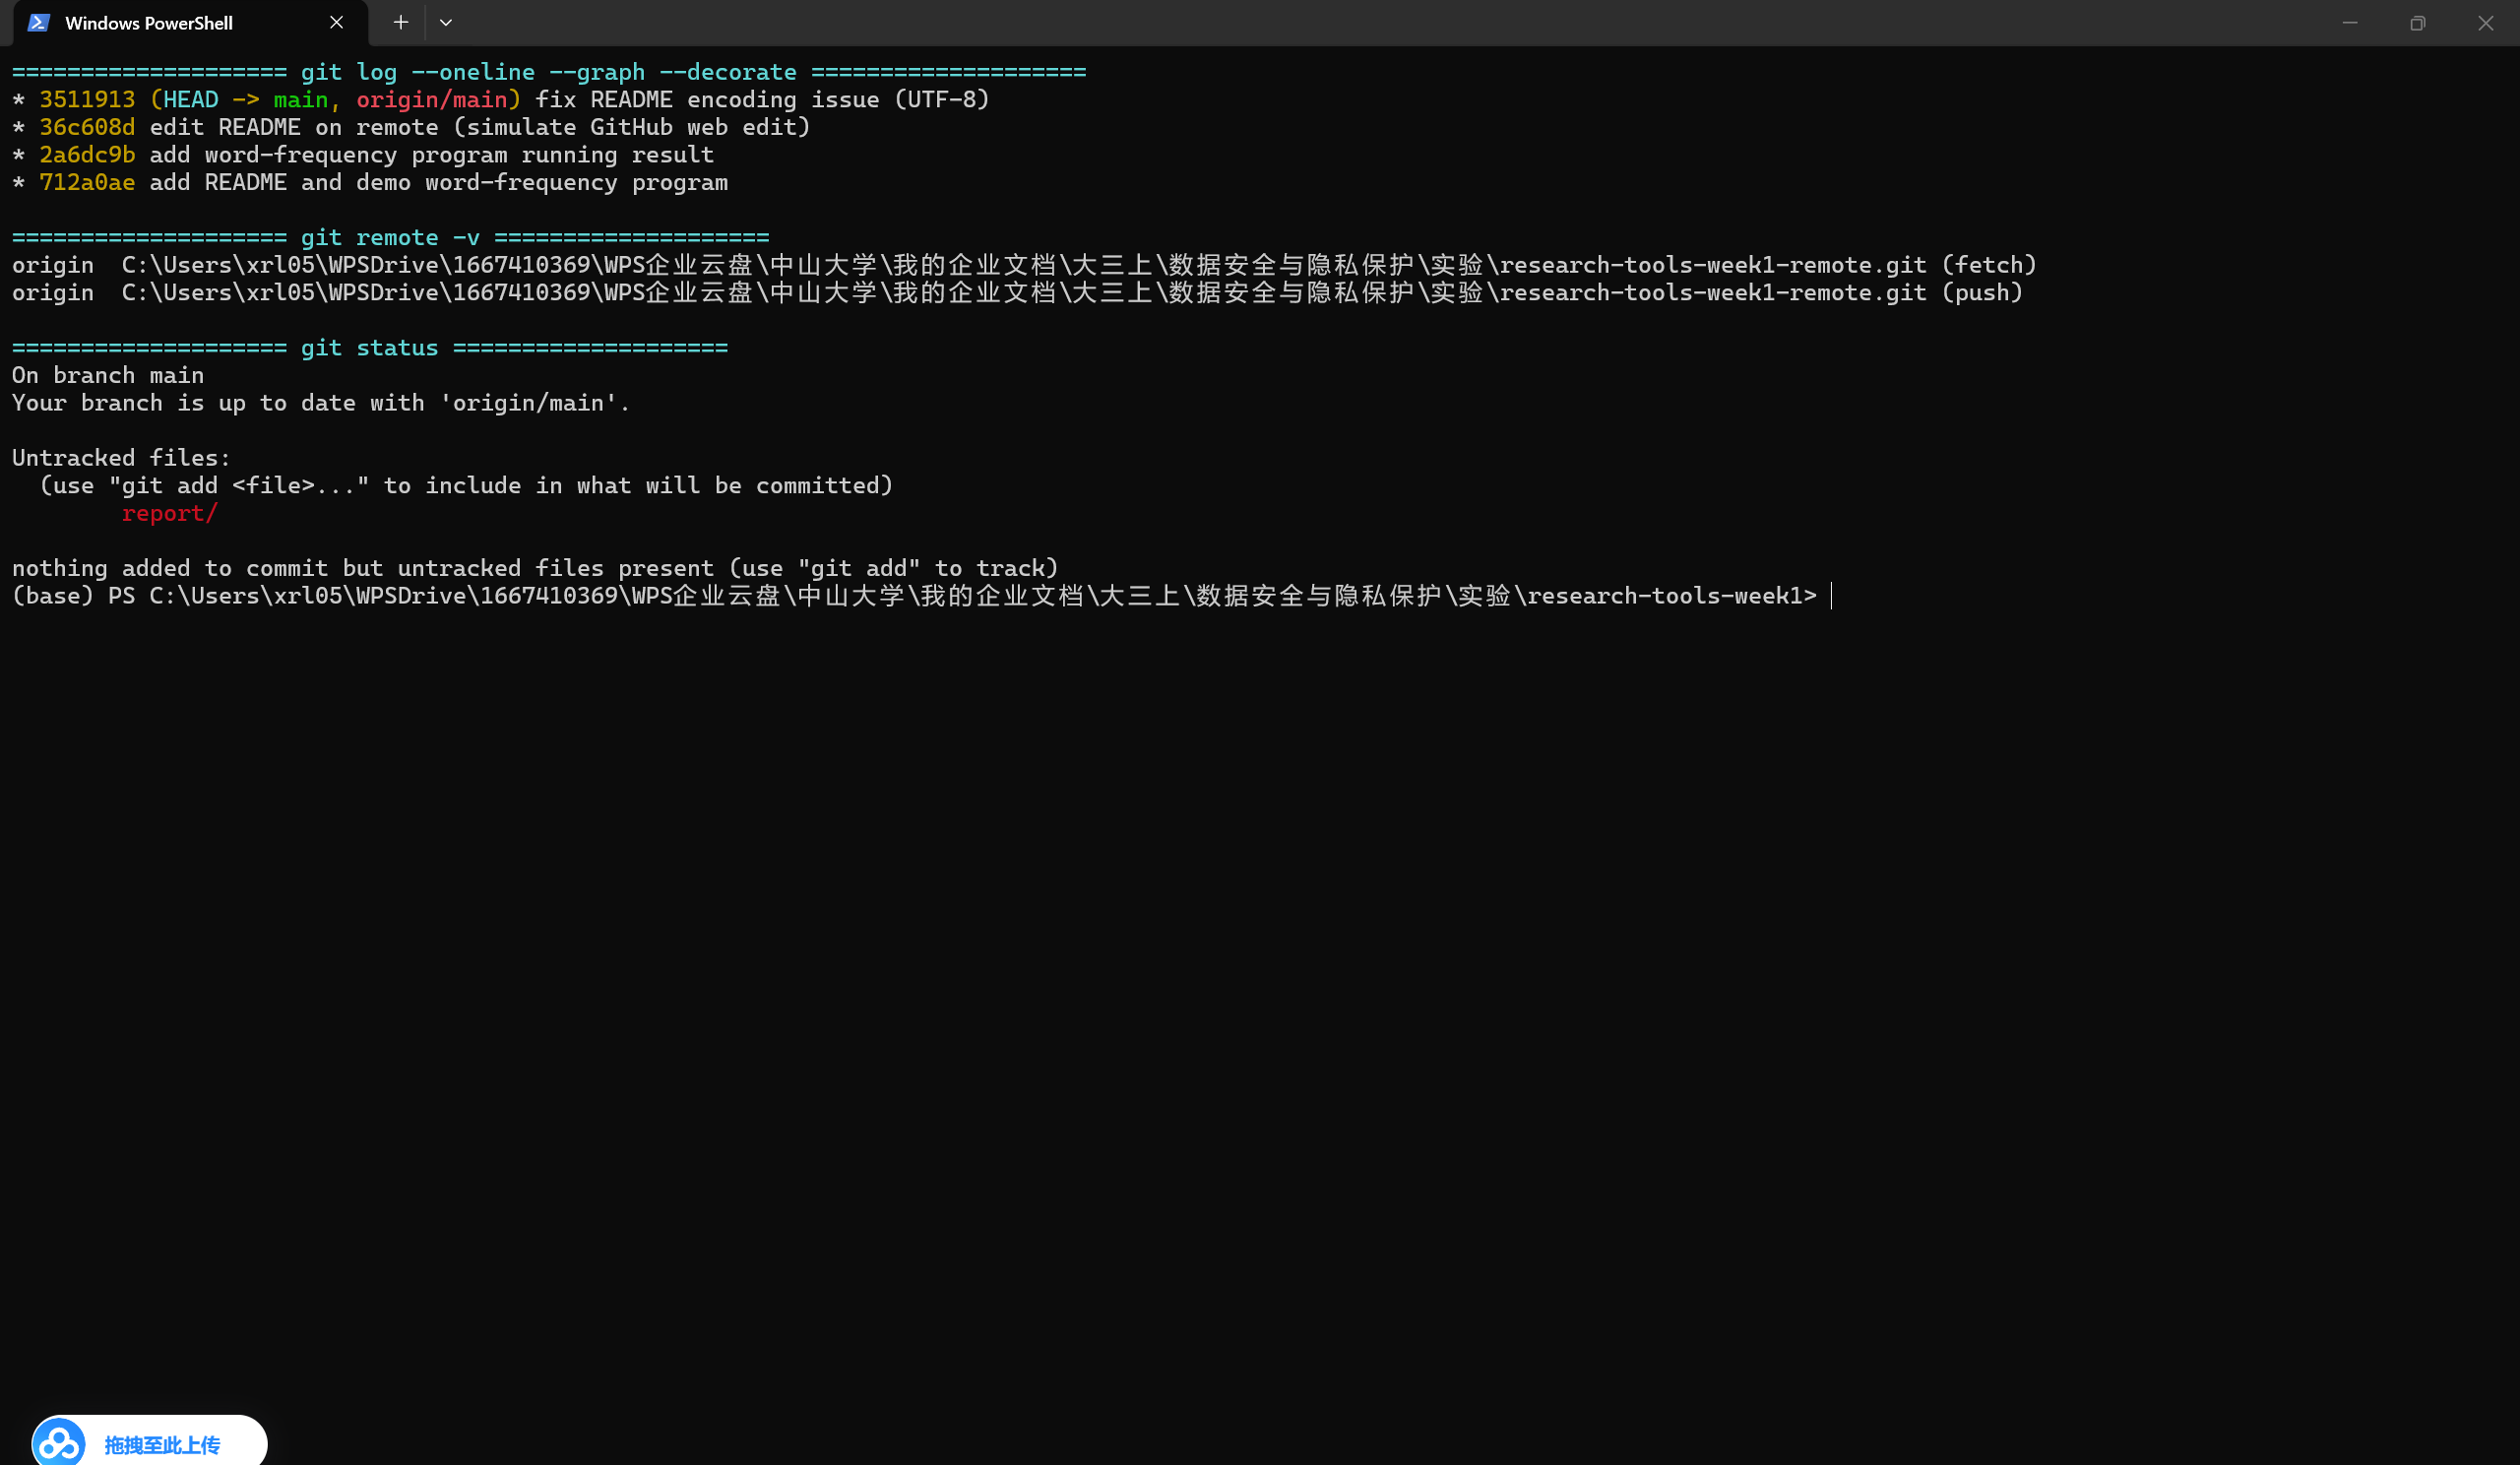
\includegraphics[width=0.95\textwidth]{figures/fig1_git.png}
    \caption{Git 提交历史、远程配置与工作区状态}
    \label{fig:git}
\end{figure}

\begin{figure}[htbp]
    \centering
    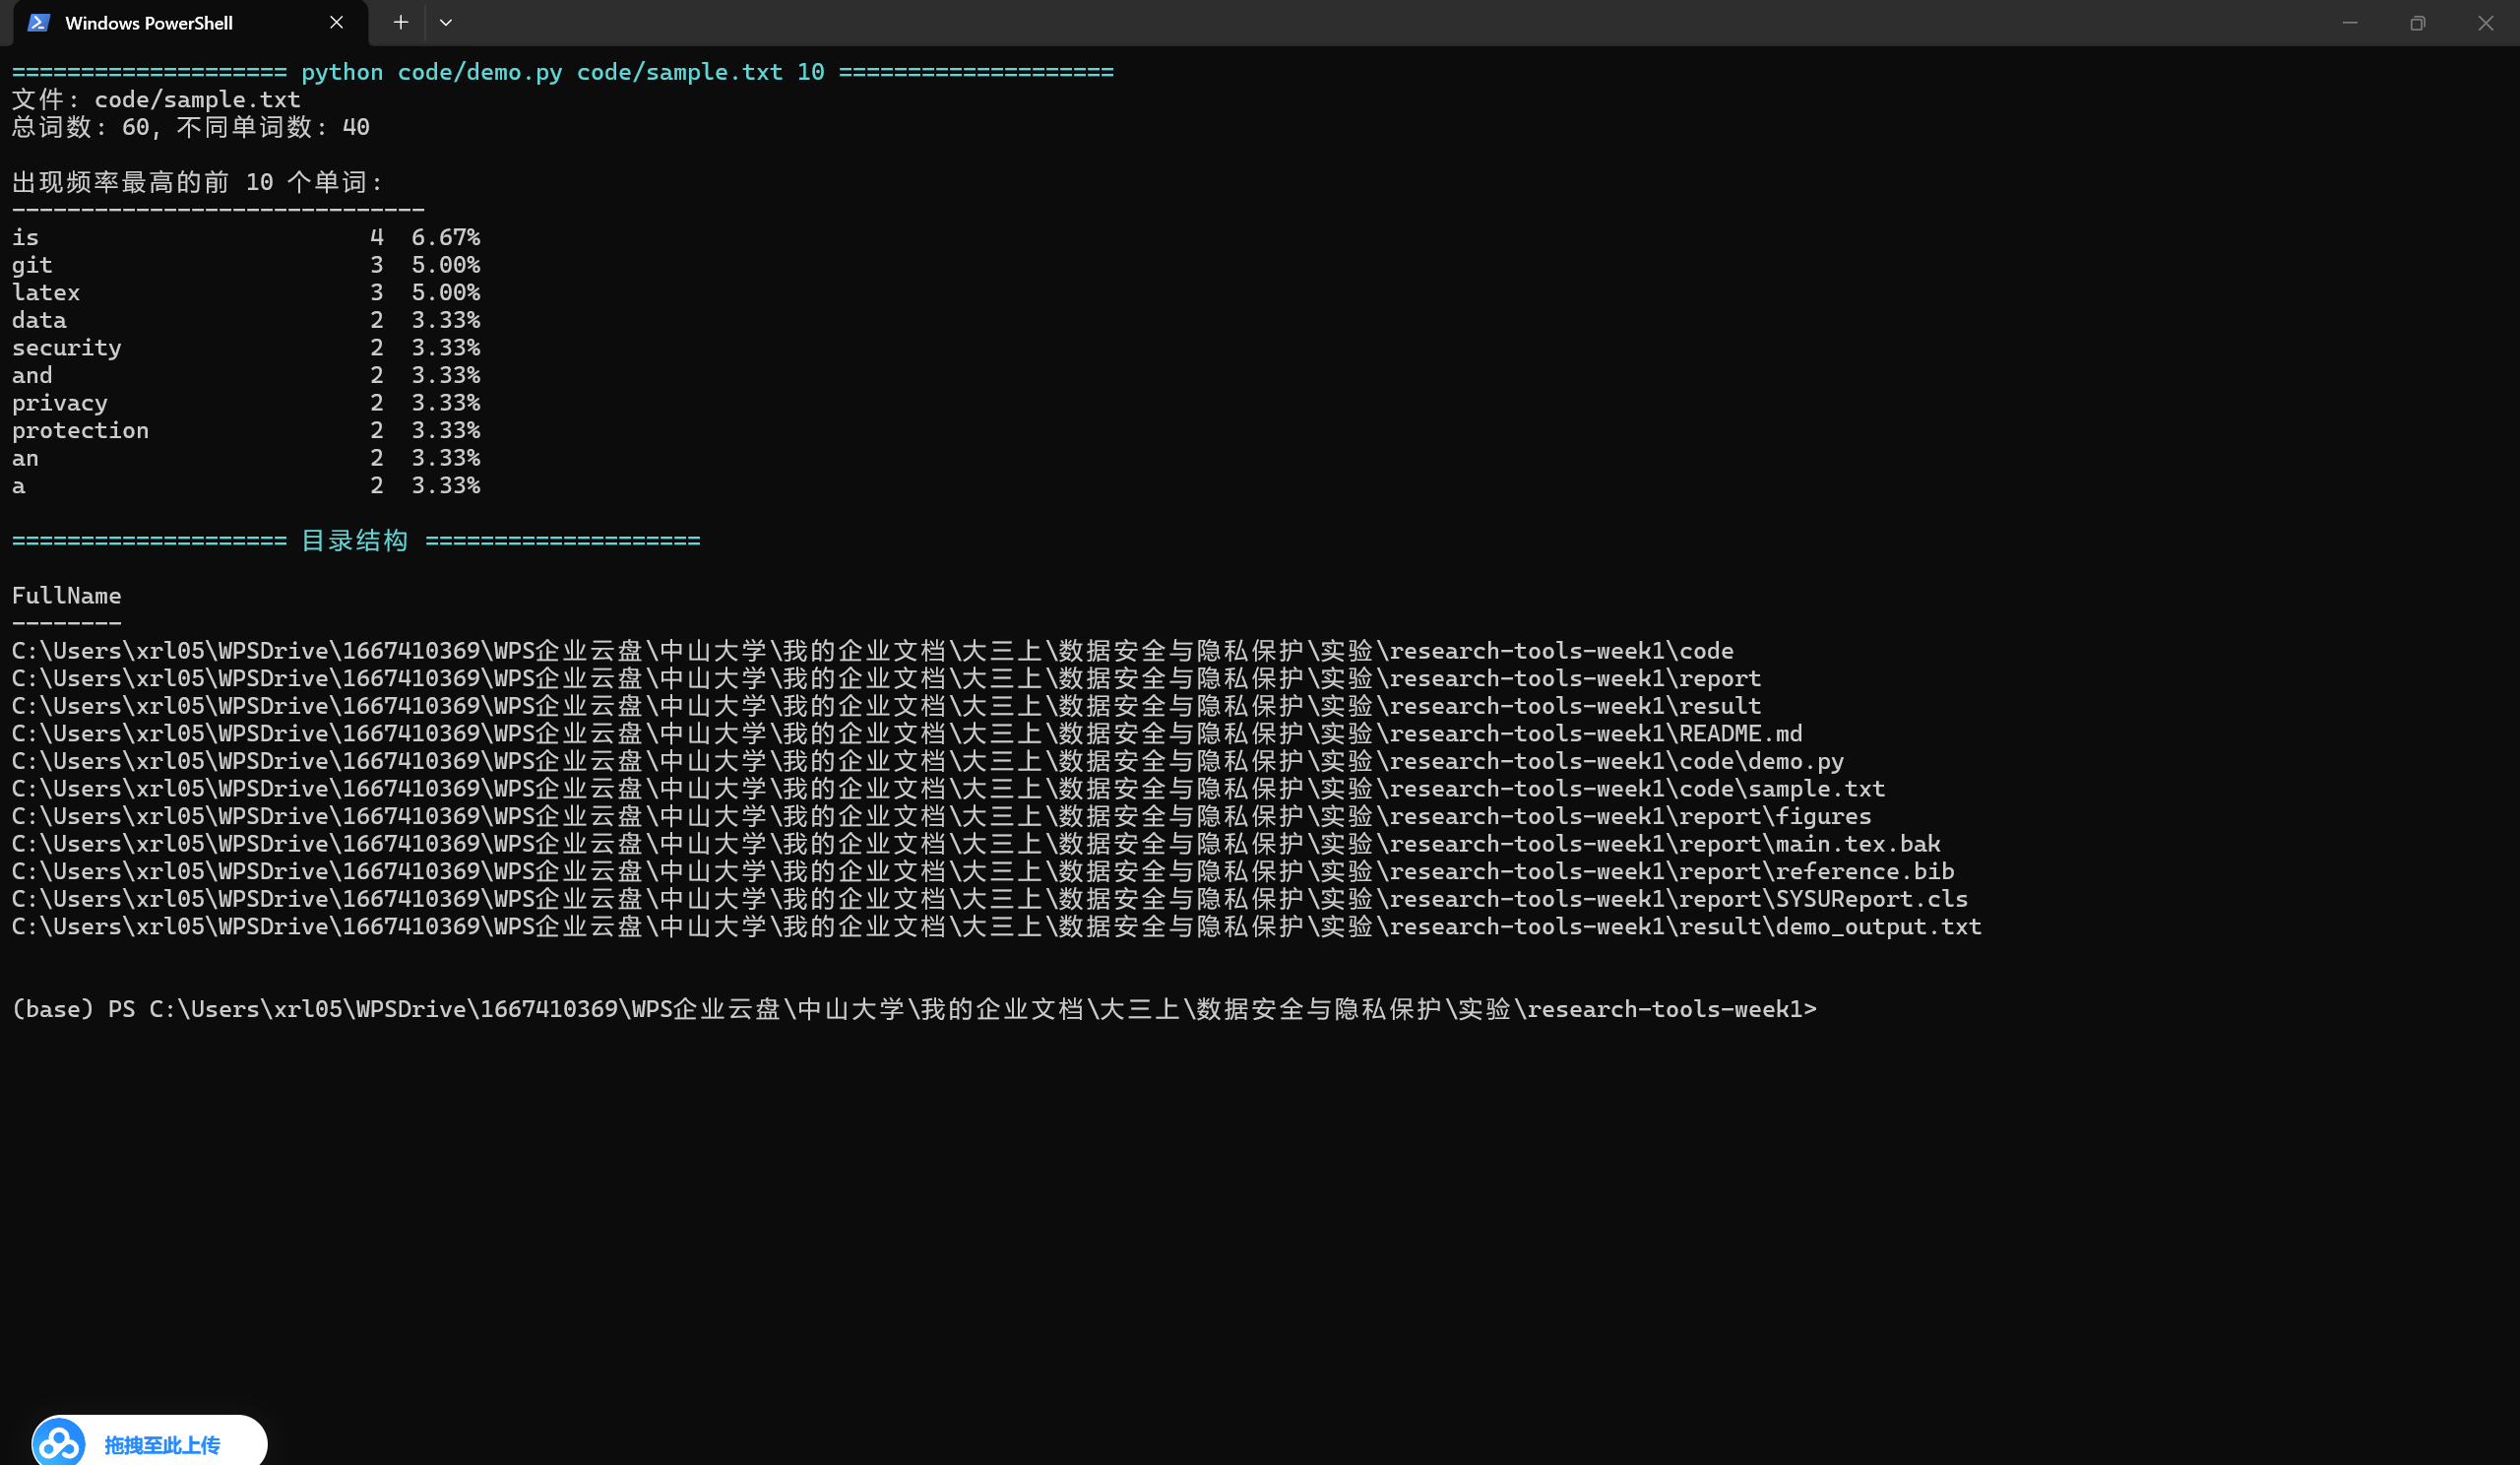
\includegraphics[width=0.95\textwidth]{figures/fig2_demo.png}
    \caption{词频统计程序运行结果与仓库目录结构}
    \label{fig:demo}
\end{figure}

\subsection{Codex 与 CC Switch 使用}

\subsubsection{安装 Codex}

本机已存在 Codex 桌面版，为获得可用的命令行环境，通过 npm 重新全局安装 Codex CLI 并确认版本：

\begin{lstlisting}[caption={通过 npm 安装 Codex CLI}]
$ npm install -g @openai/codex
added 2 packages in 2m

$ codex --version
codex-cli 0.154.0
\end{lstlisting}

\subsubsection{登录与供应商配置}

本实验采用 CC Switch v3.20.1 的 config-only 模式完成登录配置：供应商信息（端点、模型、密钥）写入 Codex 配置文件 \texttt{\textasciitilde/.codex/config.toml} 的 \texttt{[model\_providers.custom]} 表中，不再生成 \texttt{auth.json}。Codex 启动时自动读取该配置，如下所示（密钥内容不在本报告展示，防止泄露）：

\begin{lstlisting}[caption={Codex 启动时的供应商与模型配置}]
OpenAI Codex v0.153.4
--------
model: deepseek-v4-flash
provider: custom
approval: never
sandbox: read-only
reasoning effort: high
--------
\end{lstlisting}

\subsubsection{连接官方端点失败与排查}

按照实验要求，先让 Codex 阅读项目并说明目录结构，再要求其完成词频统计程序的编写。在尝试连接官方端点时，出现如下错误：

\begin{lstlisting}[caption={Codex 连接官方端点失败}]
ERROR codex_api::endpoint::responses_websocket:
failed to connect to websocket: IO error:
由于目标计算机积极拒绝，无法连接。(os error 10061)
url: wss://api.openai.com/v1/responses
ERROR: Reconnecting... waiting for network
\end{lstlisting}

经排查，原因是本机代理软件未运行（Git 全局配置中的 \texttt{http.proxy=127.0.0.1:7890} 无对应监听端口），且当前网络无法直连 OpenAI 官方端点。解决思路为：使用 CC Switch 切换到国内可直连的模型供应商（国模/中转站）。

\subsubsection{安装并配置 CC Switch}

从官方 GitHub Releases 下载 Windows 便携版 \texttt{CC-Switch-v3.20.1-Windows-Portable.zip}（12.9 MB），解压即用：

\begin{lstlisting}[caption={下载解压并启动 CC Switch}]
$ curl -L -o CC-Switch-v3.20.1-Windows-Portable.zip \
    https://github.com/farion1231/cc-switch/releases/download/v3.20.1/\
    CC-Switch-v3.20.1-Windows-Portable.zip
$ Expand-Archive CC-Switch-v3.20.1-Windows-Portable.zip portable
$ Start-Process portable/cc-switch.exe
\end{lstlisting}

启动后界面默认包含 “OpenAI Official”（官方端点）与 “default”（未配置）两个条目。配置国模供应商的步骤如下：

\begin{enumerate}
    \item 点击右上角“+”新建供应商条目；
    \item 优先选择内置预设；若自定义，按供应商文档填写名称、API Key、Endpoint URL（Codex 端点示例通常以 \texttt{/v1} 结尾）和模型；
    \item 保存后点击供应商卡片上的“启用”；
    \item 关闭并重新打开 Codex 或终端，使新的供应商和模型列表生效，再用 \texttt{/status} 和一个小问题进行验证。
\end{enumerate}

启动后界面默认包含 “OpenAI Official”（官方端点）与 “default”（未配置）两个条目。本实验在 cc-switch 中新建 DeepSeek 自定义供应商并启用：Endpoint 填写 \texttt{https://api.deepseek.com}，模型选择 \texttt{deepseek-v4-flash}，API Key 由用户在供应商平台创建并粘贴（密钥仅保存在本地配置中，不在本报告展示）。启用后 Codex 配置文件同步更新为 \texttt{model\_providers.custom}（config-only 模式，见 4.3.2 节）。

先验证供应商端点与密钥可用（密钥以环境变量传入，避免出现在命令历史中）：

\begin{lstlisting}[caption={验证 DeepSeek 供应商端点}]
$ curl -s -H "Authorization: Bearer $env:DSKEY" \
    https://api.deepseek.com/v1/models
{"object":"list","data":[
  {"id":"deepseek-flash","name":"DeepSeek-V4.1-Flash",...},
  {"id":"deepseek-v4-pro","name":"DeepSeek-V4-Pro",...}]}
# HTTP 200：端点连通、密钥有效
\end{lstlisting}

\subsubsection{任务一：Codex 只读分析项目}

配置完成后重新运行 Codex，要求其只读分析项目：

\begin{lstlisting}[caption={Codex 任务一：只读分析项目}]
$ codex exec "请先阅读项目，说明目录结构、程序入口和运行方法，不要修改任何文件。"
\end{lstlisting}

Codex 自动扫描仓库并给出结论：目录结构为 \texttt{README.md / code/(demo.py, sample.txt) / result/ / report/(LaTeX 工程)}；程序入口为 \texttt{code/demo.py}（\texttt{load\_text} 读文件、\texttt{count\_words} 正则分词计数、\texttt{main} 打印 Top-N），运行命令 \texttt{python code/demo.py code/sample.txt 10}；报告需在 \texttt{report/} 目录下用 XeLaTeX 连续编译两次。此外 Codex 还发现了两个值得注意的问题：README 快速开始命令 \texttt{python code/demo.py sample.txt} 从仓库根目录执行会因路径不存在而报错（正确应为 \texttt{code/sample.txt}）；\texttt{reference.bib} 尚未被 \texttt{main.tex} 引用，属于预留文件。由于仓库位于 WPS 云盘同步目录，Git 提示 “dubious ownership”（沙箱用户与文件属主不同），Codex 使用一次性 \texttt{-c safe.directory=...} 参数只读绕过，未写入任何全局配置。

\subsubsection{任务二：Codex 生成词频统计程序}

继续要求 Codex 编写独立的词频统计程序：

\begin{lstlisting}[caption={Codex 任务二：生成词频统计程序}]
$ codex exec "在 code/ 目录编写一个独立的文本词频统计程序 text_stats.py，
支持命令行参数（输入文本文件路径，可选 top N 参数默认 10），读取 UTF-8 文本，
统计英文单词出现次数并按频率降序输出 Top-N。只创建 code/text_stats.py。"
\end{lstlisting}

Codex 生成了完整程序（只依赖标准库，使用 \texttt{argparse} 解析参数，正则允许单词内部连字符与撇号），并因只读沙箱无法直接落盘而输出完整代码供保存；人工审阅其代码与待执行命令后，将代码保存为 \texttt{code/text_stats.py}：

\begin{lstlisting}[language=Python, caption={Codex 生成的 text_stats.py（节选）}]
import argparse, re, sys
from collections import Counter

WORD_PATTERN = re.compile(r"[A-Za-z]+(?:['\-][A-Za-z]+)*")

def count_words(text: str) -> Counter:
    return Counter(WORD_PATTERN.findall(text.lower()))

def ranking(counter: Counter, top_n: int):
    # 按次数降序、同次数按字母升序，保证输出稳定
    return sorted(counter.items(), key=lambda x: (-x[1], x[0]))[:top_n]
\end{lstlisting}

按 Codex 给出的测试方法实际运行，结果如下（正常路径、边界、异常四组）：

\begin{lstlisting}[caption={text_stats.py 测试结果}]
$ python code/text_stats.py code/sample.txt          # 默认 Top-10
文件: code/sample.txt
总词数: 60, 不同单词数: 40
出现频率最高的前 10 个单词
----------------------------------------
is                        4  6.67%
git                       3  5.00%
latex                     3  5.00%
...

$ python code/text_stats.py tmp_words.txt -n 3        # 边界：大小写/撇号/连字符
文件: tmp_words.txt
总词数: 8, 不同单词数: 5
world                     3  37.50%
hello                     2  25.00%
e-mail                    1  12.50%

$ python code/text_stats.py no_such_file.txt          # 异常：文件不存在
错误: 找不到文件 no_such_file.txt    （退出码 2）
$ python code/text_stats.py code/sample.txt -n -1     # 异常：负数
text_stats.py: error: top N 不能为负数    （退出码 2）
\end{lstlisting}

默认 Top-10 结果与 \texttt{demo.py} 输出交叉验证一致（总词数 60、不同单词 40，最高频 \texttt{is} 出现 4 次占 6.67\%），边界与异常用例均符合预期，退出码正确。

随后用 Git 独立检查 Codex 的修改：\texttt{git status} 确认仅有 \texttt{code/text_stats.py} 一个新增文件，审阅 \texttt{git diff} 无误后提交并推送真实 GitHub 远程：

\begin{lstlisting}[caption={Git 复核并提交推送}]
$ git status
Untracked files:
	code/text_stats.py
$ git add code/text_stats.py
$ git commit -m "add text_stats.py generated by Codex with tests"
[main 2cda0fb] add text_stats.py generated by Codex with tests
 1 file changed, 96 insertions(+)
$ git push github main
   8cf6bb6..2cda0fb  main -> main
\end{lstlisting}

至此，“Codex 完成至少一次任务（代码阅读、生成或修改）”的要求已全部完成：任务一完成代码阅读与分析，任务二完成程序生成、测试验证与提交推送。

\section{实验总结}

通过本次实验，我系统完成了科研基础工具的练习：

\begin{enumerate}
    \item \textbf{Git 与 GitHub}：掌握了仓库初始化（\texttt{git init}）、暂存与提交（\texttt{add/commit}）、历史查看（\texttt{log}）、远程同步（\texttt{push/pull}）的完整流程，养成了“开始工作先 pull，修改后看 status 和 diff，确认后 add、commit，结束再 push”的固定节奏。实验中通过本地裸仓库模拟了 GitHub 远程操作，流程与真实远程完全一致；还实践了“一次提交一个清晰目标、提交说明用动词”等良好习惯。
    \item \textbf{LaTeX 图片规范}：掌握了 \texttt{graphicx}、\texttt{figure} 环境、\texttt{caption} 图题与 \texttt{label/ref} 交叉引用的用法，并实际将词频统计结果导出为 PDF 矢量图插入报告，理解并践行了“优先使用矢量图、避免低分辨率截图”的原则。
    \item \textbf{AI 辅助编程工具}：完成了 Codex CLI 的安装与配置，理解并实践了其“权限确认—命令审阅—运行测试—Git 复核”的可靠使用流程；通过 CC Switch 将供应商切换为国内可直连的 DeepSeek，成功完成“项目只读分析”和“生成词频统计程序并测试”两项任务，并提交推送至真实 GitHub 仓库。过程中还认识到：外网不可达时，合理配置国内模型供应商/中转是保证科研工具可用的有效途径。
    \item \textbf{遇到的问题与解决}：① 官方端点连接失败——通过 CC Switch 切换国内供应商（DeepSeek）解决；② DeepSeek 旧密钥失效（401）——在供应商平台重新创建密钥并更新配置后解决；③ Windows 下 Git 的 LF/CRLF 换行符警告——属正常现象，不影响功能；④ 脚本写入 README 导致中文乱码——统一使用 UTF-8 编码并修复提交；⑤ PowerShell 控制台中文路径乱码——设置 \texttt{chcp 65001} 与 UTF-8 输出编码解决。
\end{enumerate}

总体而言，本次实验为后续课程的代码管理与实验报告撰写打下了规范基础，我将在后续实验中保持“可复现、可追溯、规范保存”的习惯。

\end{document}
